\documentclass[10pt,a4paper]{report}
\usepackage[utf8]{inputenc}
\usepackage[francais]{babel}
\usepackage{xcolor}
\usepackage{graphicx}
\usepackage{amsmath,amsfonts,amssymb}

\date{\today}

\begin{document}

\title{Rapport d'Analyse Syntaxique et Projet de Programmation}

\author{Claude Cugerone, Bérénice Faltrept, Amélie Guémon, Marin Liebert}

\tableofcontents

\section{Introduction}

Le but du projet était de créer un analyseur syntaxique qui vérifie la syntaxe d'un code C et d'un fichier LateX. Les fichiers traités seraient ensuite retranscrits en pages html, à la manière d'un site. Ce logiciel devra être capable de générer notre rapport de projet à partir d'un fichier lateX.
Ce site rapporte le travail effectué durant la période donnée pour réaliser ce projet et des exemples d'utilisation. 
Un menu en haut de chaque page permet de naviguer sur les différentes partie du projet :
\begin{itemize}
\item {\bf Une partie C} montrant la transcription d'un fichier .c sur une page Html.
\item {\bf Une partie Documentation} qui se charge de documenter le fichier .c
\item {\bf Une partie LateX} dans laquelle vous trouverez le rapport généré à partir d'un fichier LaTeX

Nous avons aussi écrit un script simple vous permettant de compiler puis lancer nos analyseurs latex et c sur nos fichiers de tests et ainsi de générer les fichiers formant le site web. \\

\section{Analyse de la partie C}

Le parseur ne permet pas de générer à partir d'un document de la taille de notre rapport. Nous avons donc généré des pages séparées pour cette section, et celle de latex.

\section{Partie Doxygen}

Les commentaires Doxygen servent à documenter un fichier C. La documentation est générée sous forme html. Elle a pour syntaxe :
\newline
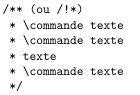
\includegraphics{code1.png}

Les commandes Doxygen reconnues par notre projet sont : fn, brief, param et return. Une commande et son texte peuvent prendre une ou plusieurs ligne comme dans l'exemple ci-dessus.

La documentation est analysée, puis elle est générée en syntaxe html avec le css adéquat.

\subsection{Problèmes rencontrés}
Nous avons eu des problèmes sur la manière de reconnaître les différents motifs dans un commentaire doxygen car il n'y avait pas une ligne pour une commande. Finalement nous avons crée une "commande actuelle" qui se met à joue seulement quand il y a une nouvelle commande de lue.


\subsection{Améliorations possibles}
Une amélioration possible serait que l'analyseur récupère toutes les prototypes de fonction dans le .h et qu'il génère un début de commentaire doxygen avec les bonnes balises en fonction du nombre de paramètres de la fonction. L'utilisateur n'aurait plus qu'à rajouter son texte.

Une autre amélioration serait de gérer les balises-liens entres les descriptions de fonctions afin de faciliter le déplacement et la lecture de la documentation par l'utilisateur.








\section{Conclusion}
Nous avons rencontré plusieurs problèmes lors de la fusion de nos différents travaux.

Nous remercions nos encadrants de nous avoir proposé un sujet aussi complet et intéressant à réaliser, et nous regrettons de ne pas avoir plus de temps pour le compléter.


\includegraphics{Mini_Amel.png}

\end{document}
